\section{Detector geometry}
\label{sec:geometry}

In this section we describe the relevant components of the detector and their relations.

The detector is made of two identical modules
identified by their relative geographic location
as \emph{East} (\Module{E}) and \emph{West} (\Module{W}) module (\cref{fig:chimneys}).
As a reminder, the orientation is such that the Booster Neutrino Beam impinges
upon the detector from the south side.

\begin{figure}[bt] % [p]
%   \centering{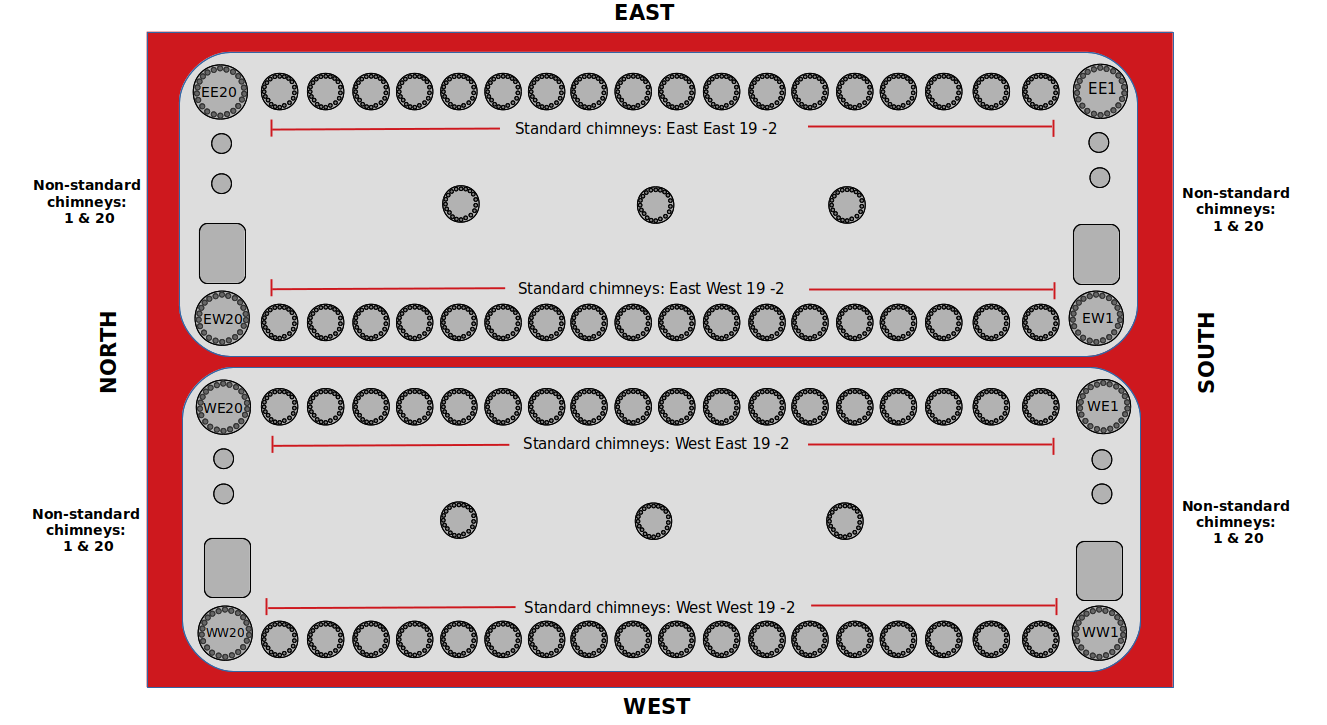
\includegraphics[width=0.90\textheight,angle=270]{figures/Icarus_chimneys}}
  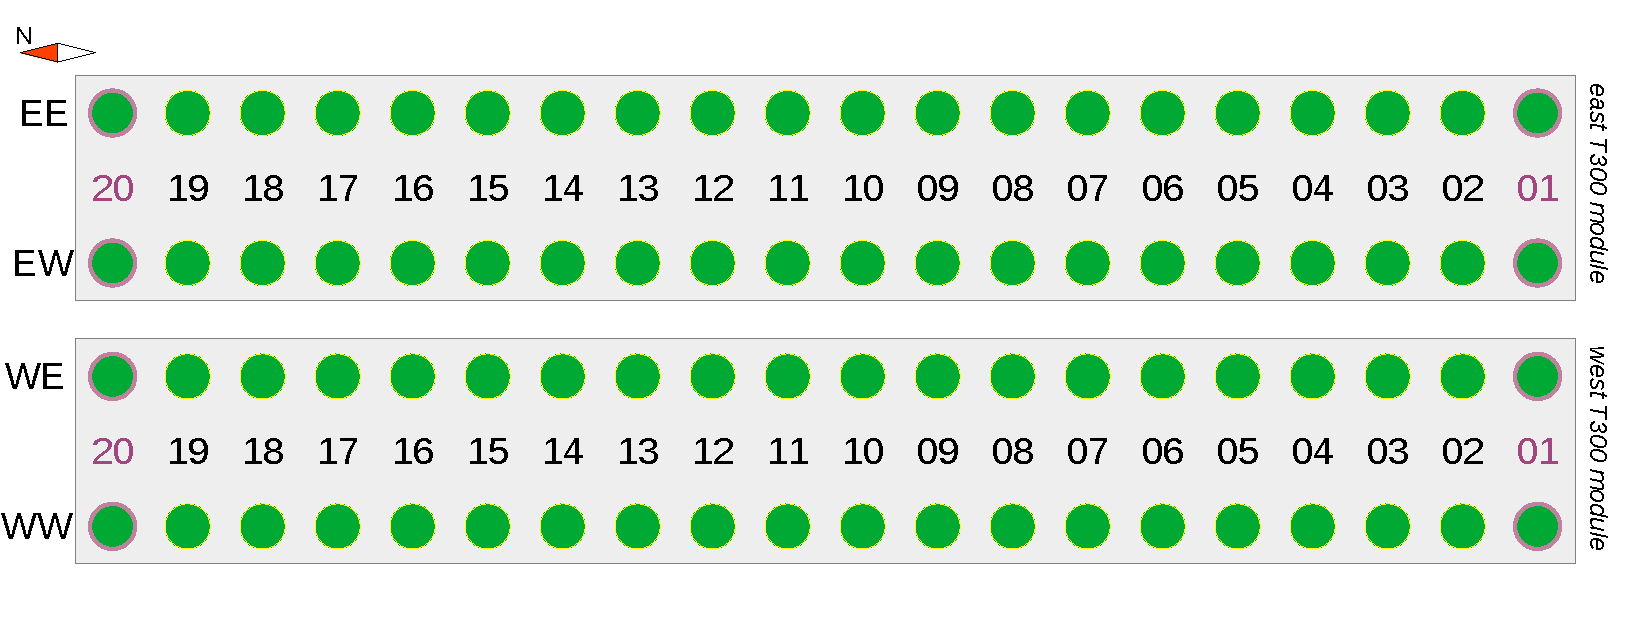
\includegraphics[width=\textwidth]{figures/ChimneyMap}
  \caption{
    Disposition of the chimneys on the top of ICARUS detectors (from~\cite{SBNDocDB14316}; see also~\cite{SBNDocDBxxxx:ConnTest}).
    \label{fig:chimneys}
  }
\end{figure}

In the following text we'll describe module \Module{E},
with the understanding that the same considerations apply to module \Module{W} as well.


\subsection{TPC wires}
\label{ssec:geometry:wires}

The module internally presents the vertical cathode in the middle, shared by
the two TPC, \TPC{EW} and \TPC{EE}.
The frame of the anodes pins the TPC wires on three different planes.
As shown in \cref{fig:WirePlanesInTPC}, the most internal of the planes,
the \emph{first induction plane}, has horizontal wires crossing the anode frame.
These wires are actually about \meter{9} long,
with one end soldered to one of the vertical short sides of the anode frame
and the other end pinned in the middle of the frame.
We can label them as ``north wires'' or ``south wires''
according to the side of the anode frame they are connected to.
These wires are connected via 68-pin flat cables to the top and middle flange
of the closest end chimney.
The cables have tag
\CableTag{C} (\texttt{EE01} and \texttt{WE01}),
\CableTag{D} (\texttt{EE20} and \texttt{WE20}),
\CableTag{A} (\texttt{EW01} and \texttt{WW01})
and
\CableTag{B} (\texttt{EW20} and \texttt{WW20}).

The other two planes have most of the wires soldered at the top and the bottom of the anode frame
(\centim{365.8} long).
These wires are connected to the 68-pin cables on the top side of the anode frame.
Other wires are soldered at the top and at a side of the frame:
these shorter wires are also connected to the cables on the top side of the anode frame.
The cables from both these groups of wires lead to the single flange of the closest of the standard chimneys.
Finally, the rest of the wires are soldered at the side and the bottom of the anode frame.
The cables of these wires, attached to the side of the frame,
lead to the bottom flange of the closest end chimney.

There are two relevant exceptions to this pattern.
Since each plane turns out to have an odd number of 68-pin cables,
but the readout boards serve two cables each,
some of the readout boards have only half the channels physically connected to a cable,
with the other half being ``ghost''.
The top flanges of all end chimneys host only eight readout board,
the ninth slot in the readout crate being empty
because no cables are connected there.
These holes are assigned channel numbers as if there were readout boards in them,
but the resulting 64 channels are also considered ``virtual'' channels.
In addition, in the corners where wires would be the shortest
(in second induction and collection planes) the wires are replaced by triangular
plates and the 68-pin cable which reach there are not connected to any wire.
These plates cover two cables each, giving rise to 64 ``wireless'' channels on
each corner, 128 on each of those planes.


\subsection{Flanges}

Each of the flanges on the standard chimneys serves
nine cables from the second induction plane
and nine cables from the collection plane.
The connectors are deployed in a $9 \times 2$ array (\cref{fig:FlangeStandard}).

\begin{figure}
  % we haven't assigned captions and labels to the subfigures,
  % so it does not make sense to reference them directly
  \begin{subfigure}{0.45\linewidth}
    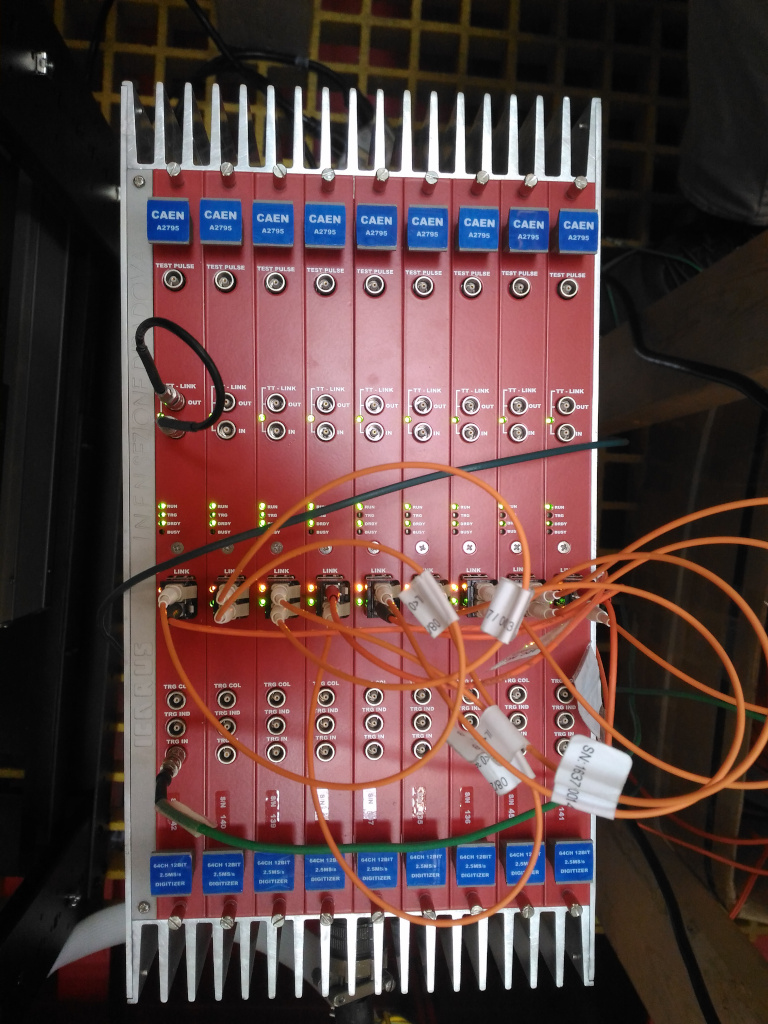
\includegraphics[width=\textwidth]{figures/ReadoutCrate-standard}
%     \label{fig:StandardMinicrate}
  \end{subfigure}
  \begin{subfigure}{0.55\linewidth}
    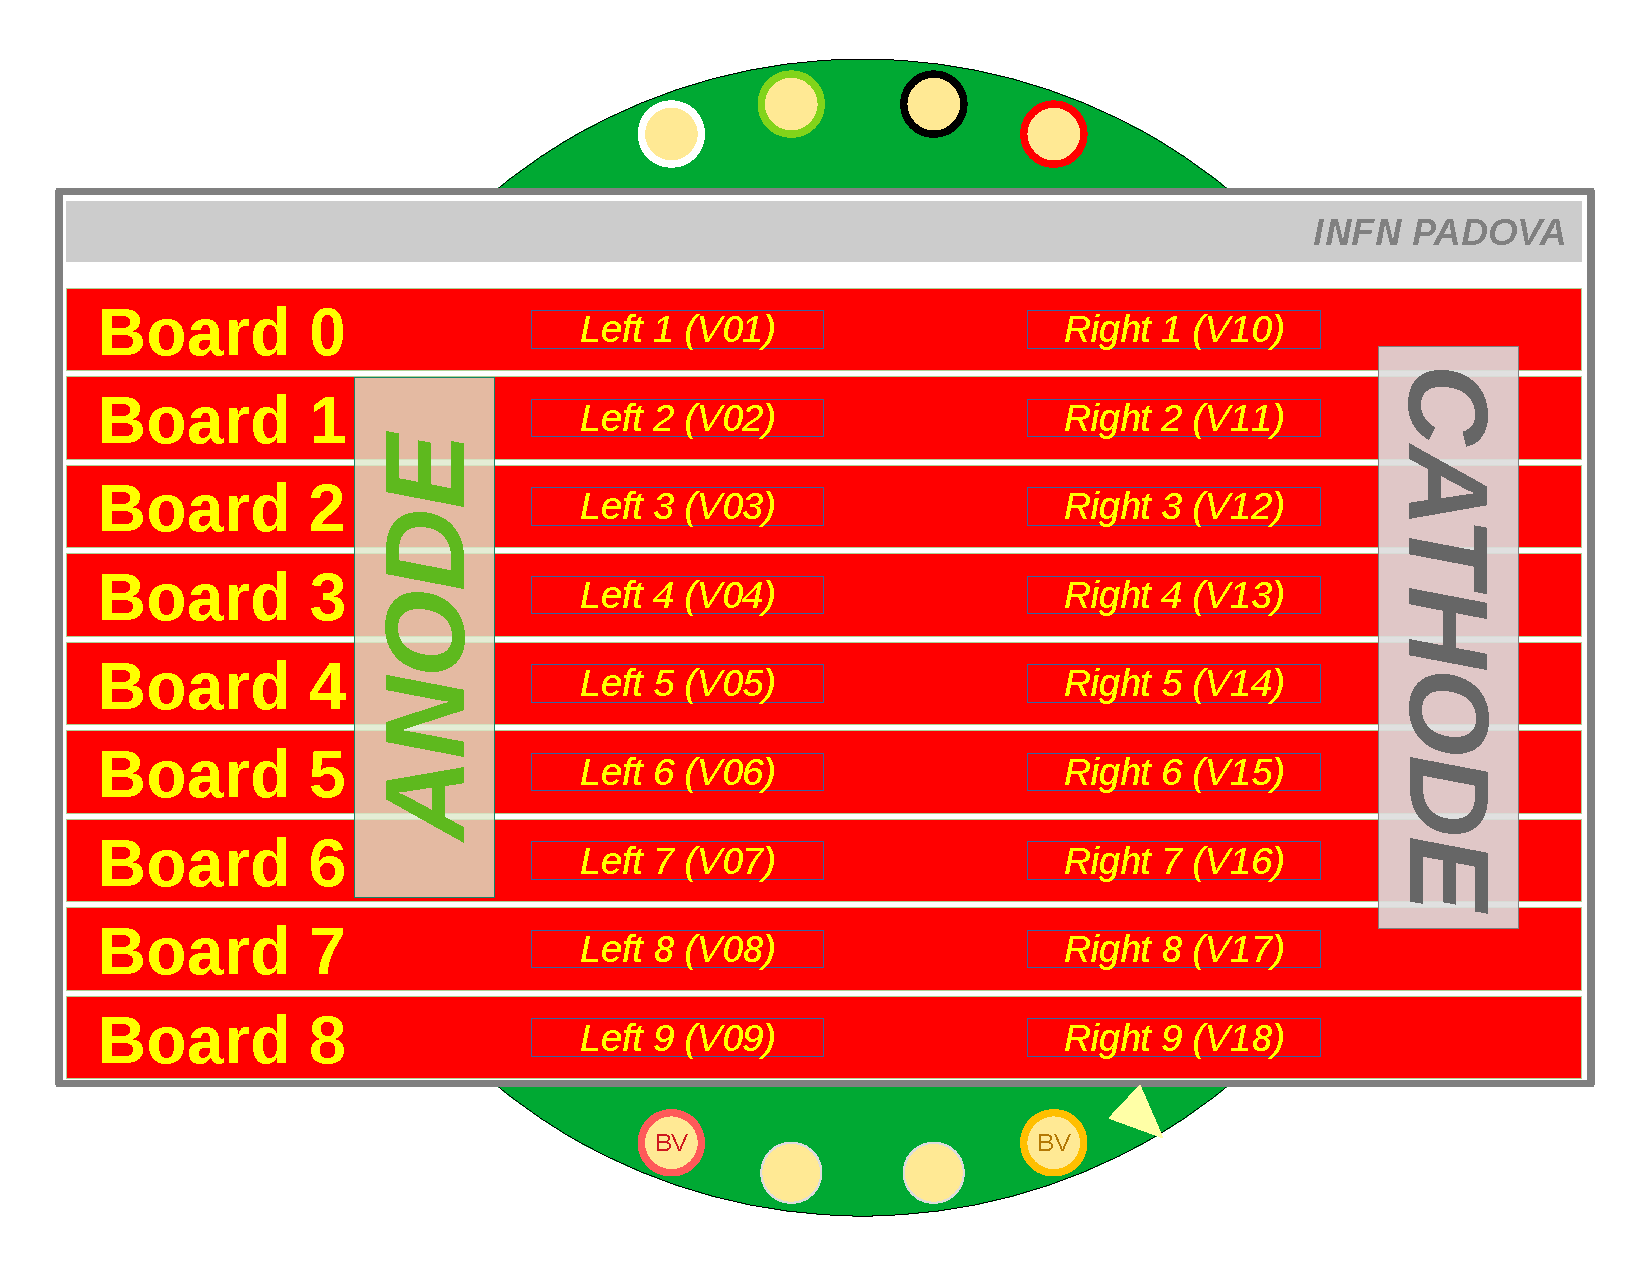
\includegraphics[width=\textwidth]{figures/TopFlangesAndMinicrate}
%     \label{fig:FlangeConnectionsStandard}
  \end{subfigure}
  \caption{
    Picture and illustration of the connections on top of a flange on a standard chimney.
    The orientation is set by the reference mark,
    the yellow triangle on the top right,
    which is pointing toward the side of the cathode
    (\ie westward for \TPC{E} TPCs and eastward for \TPC{W} TPCs).
  }
  \label{fig:FlangeStandard}
\end{figure}

These cables may come with a \CableTag{V} or \CableTag{S} tag, depending on the TPC.
Their cables are numbered from 1 to 18 (\eg \Cable{S13}):
the assignment of cables to wire planes is still under consideration due to some conflicting evidence (see \ref{ssec:PlaneAssignment} for more details and references). 

The eight end chimneys are more varied, each one with three flanges.
The top two flanges (``top'' and ``middle'') serve the first induction plane,
while each of the bottom ones serves one of the other two planes.

The minicrates on these flanges are identical to the ones on the standard chimneys,
with the connectors still deployed in a $9 \times 2$ array
(\cref{fig:FlangeConnectionsCorner})
but with different connection patterns.

\begin{figure}
  \begin{subfigure}{0.45\linewidth}
    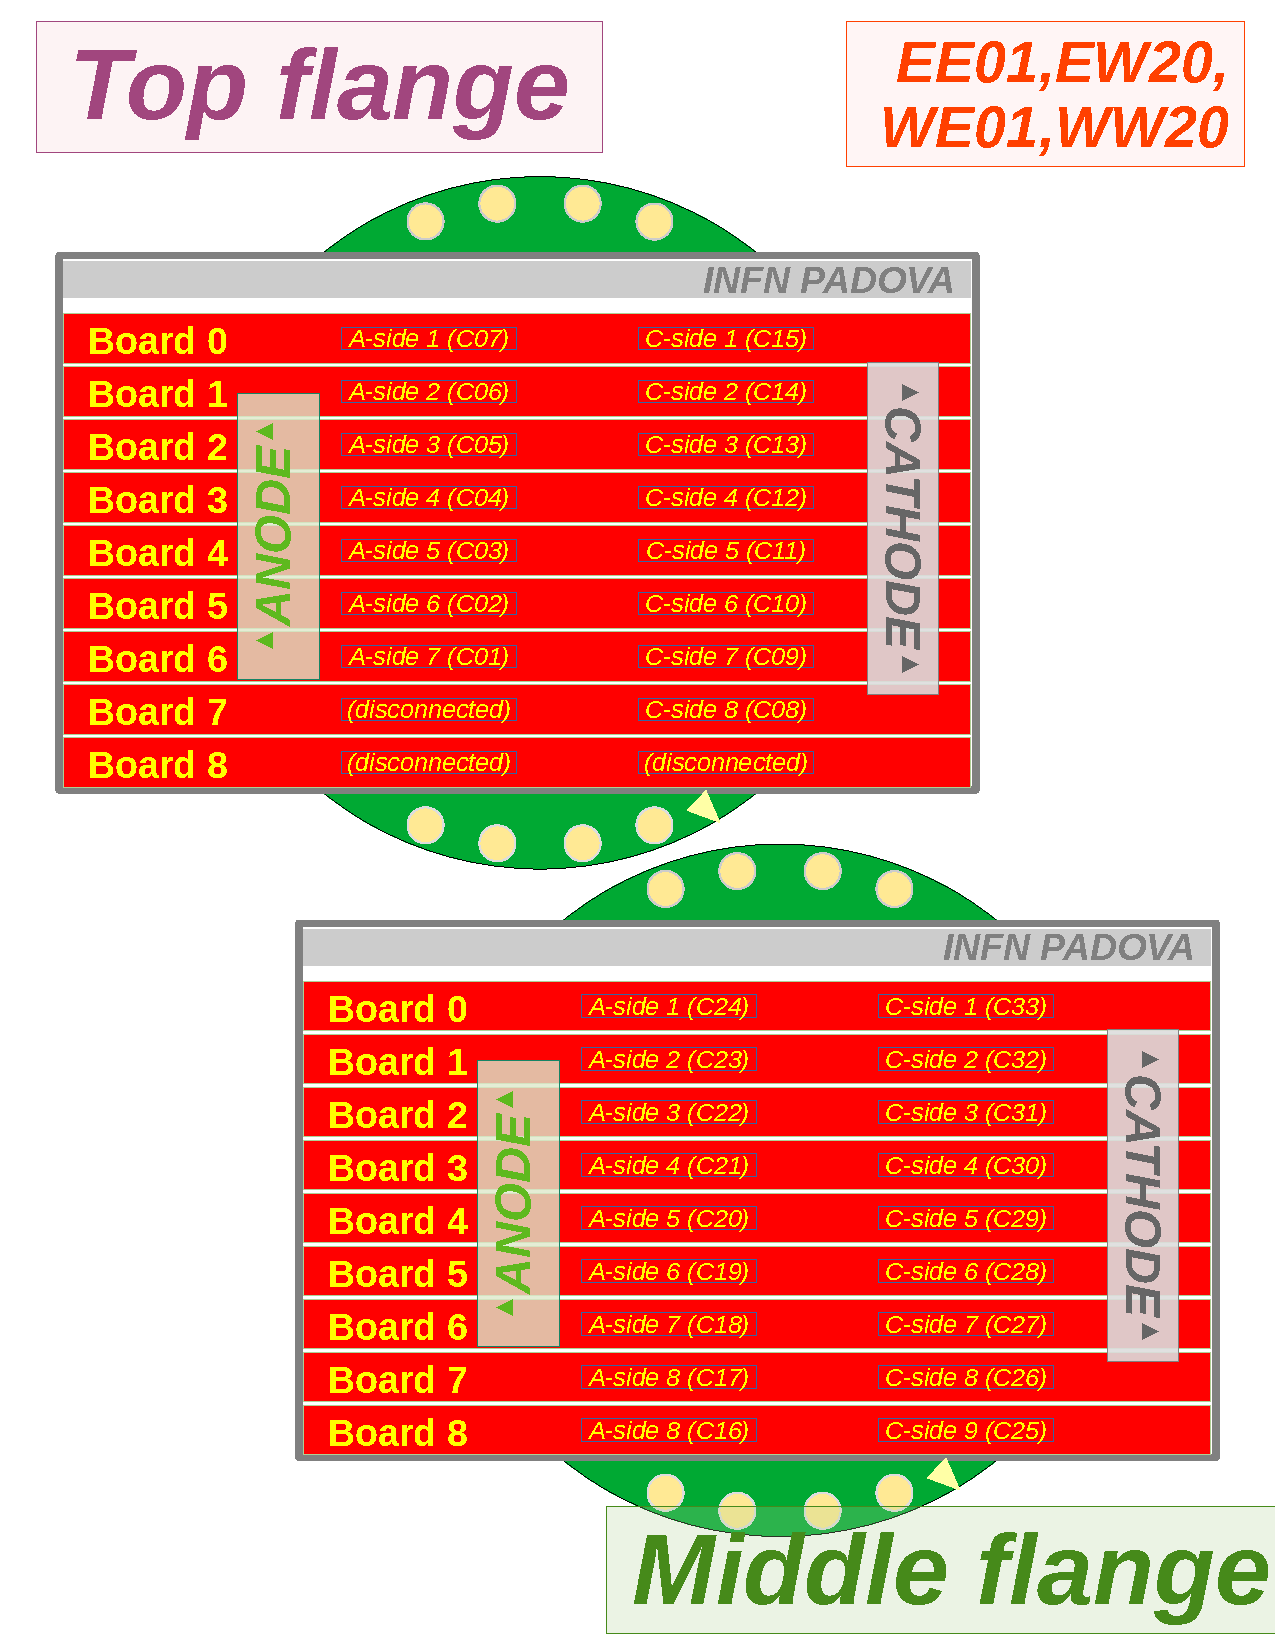
\includegraphics[width=\textwidth]{figures/CornerFlangesAndMinicrate_upward}
    \caption{Actual cable tags: \CableTag{A} (\Chimney{xW20}), \CableTag{C} (\Chimney{xE01}).}
    \label{fig:FlangeConnectionsCorner_upward}
  \end{subfigure}
  \begin{subfigure}{0.45\linewidth}
    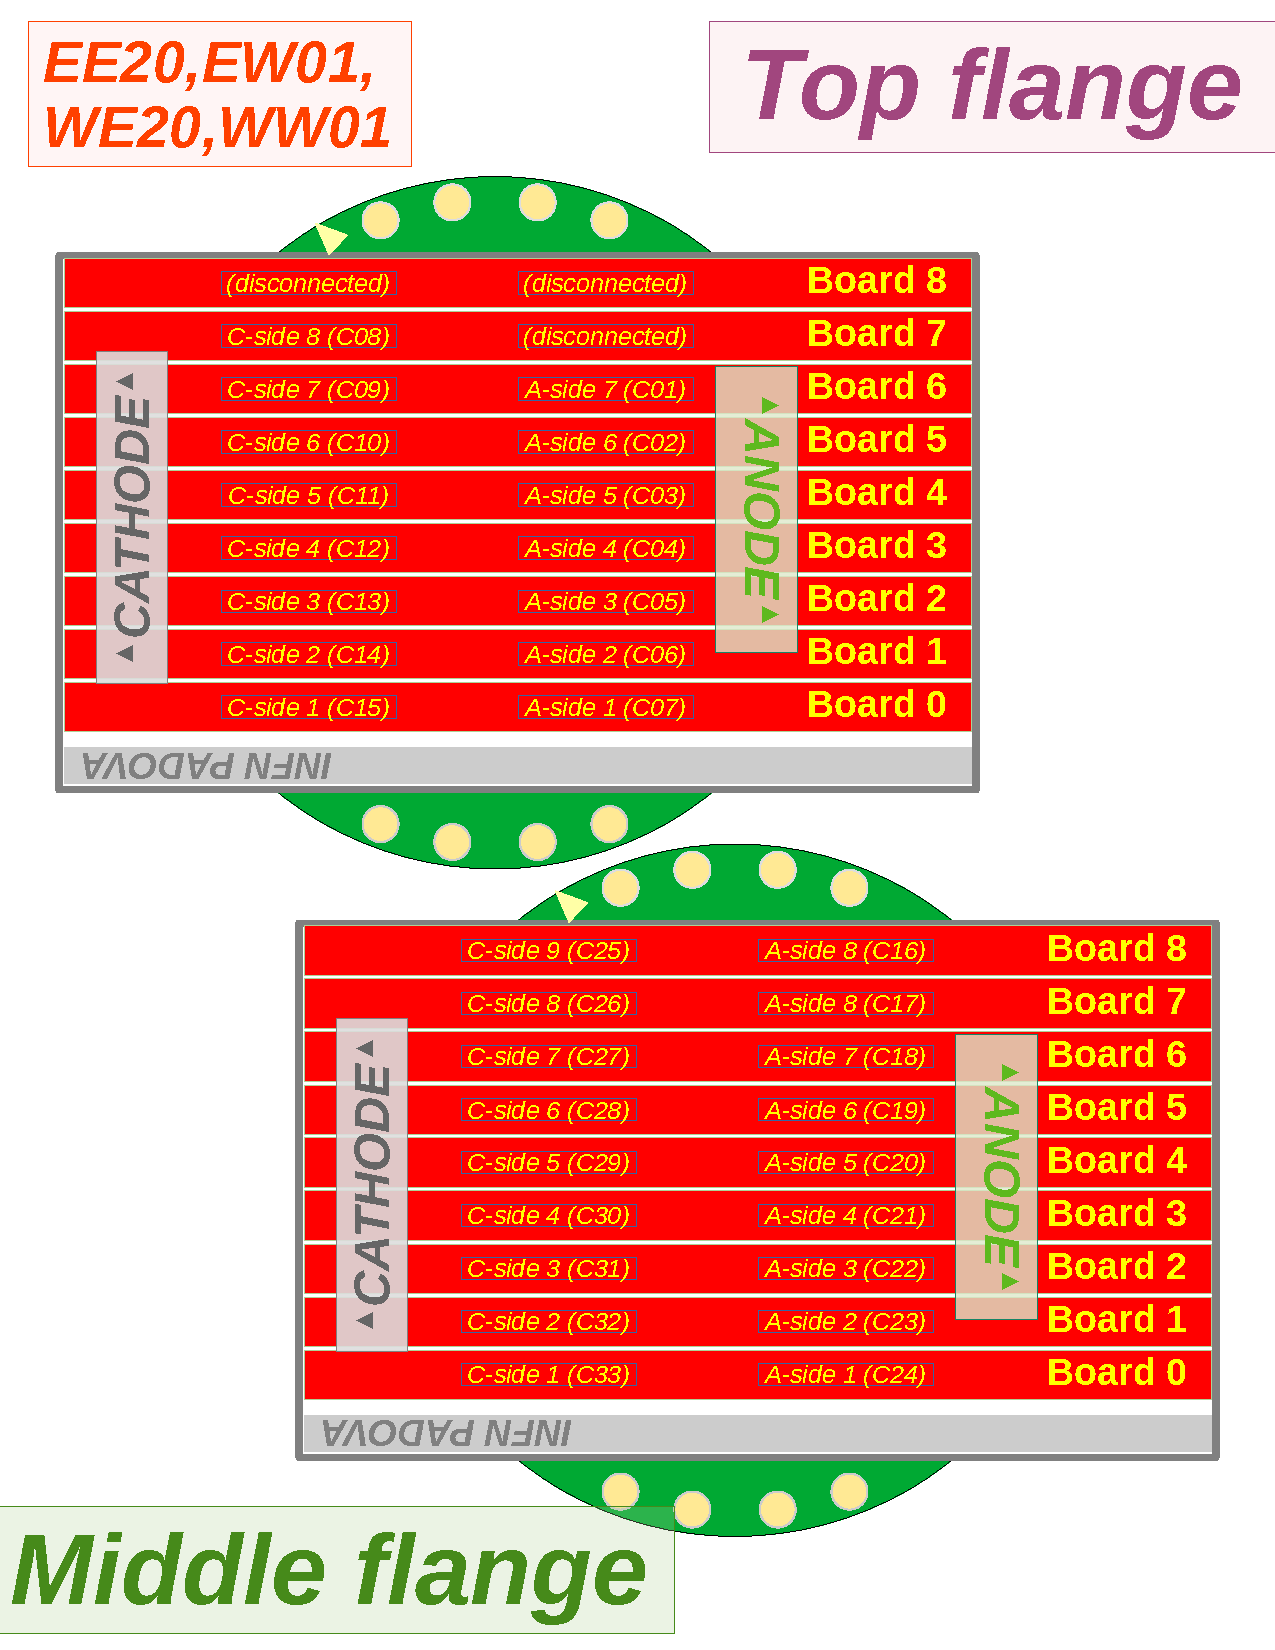
\includegraphics[width=\textwidth]{figures/CornerFlangesAndMinicrate_downward}
    \caption{Actual cable tags: \CableTag{B} (\Chimney{xW01}), \CableTag{D} (\Chimney{xE20}).}
    \label{fig:FlangeConnectionsCorner_downward}
  \end{subfigure}
  \caption{
    Illustration of the connections on top of a flange on a end chimney.
    The orientation is set by the reference mark.
    To the observer standing in front of the chimney,
    the minicrates of half the chimneys look upside down.
    The yellow triangle still points toward the side of the cathode
    (\ie westward for \TPC{E} TPCs and eastward for \TPC{W} TPCs).
  }
  \label{fig:FlangeConnectionsCorner}
\end{figure}

The labelling looks different for end chimneys at different locations.
To better understand their orientation,
it is important to consider that the physical minicrate has one side
(with fans and power supply connection) which is always oriented toward the border of its module (\ie toward the anode).
Since on the two ends of the TPC the flanges are rotated by the right angle around the east-west direction ($x$ direction),
one clockwise and the other counterclockwise,
the effect is that to the standing observer they look one upside down respect to the other.
Removing this effect, though, they are actually placed in the same way.



\begin{figure}[p]
  \centerline{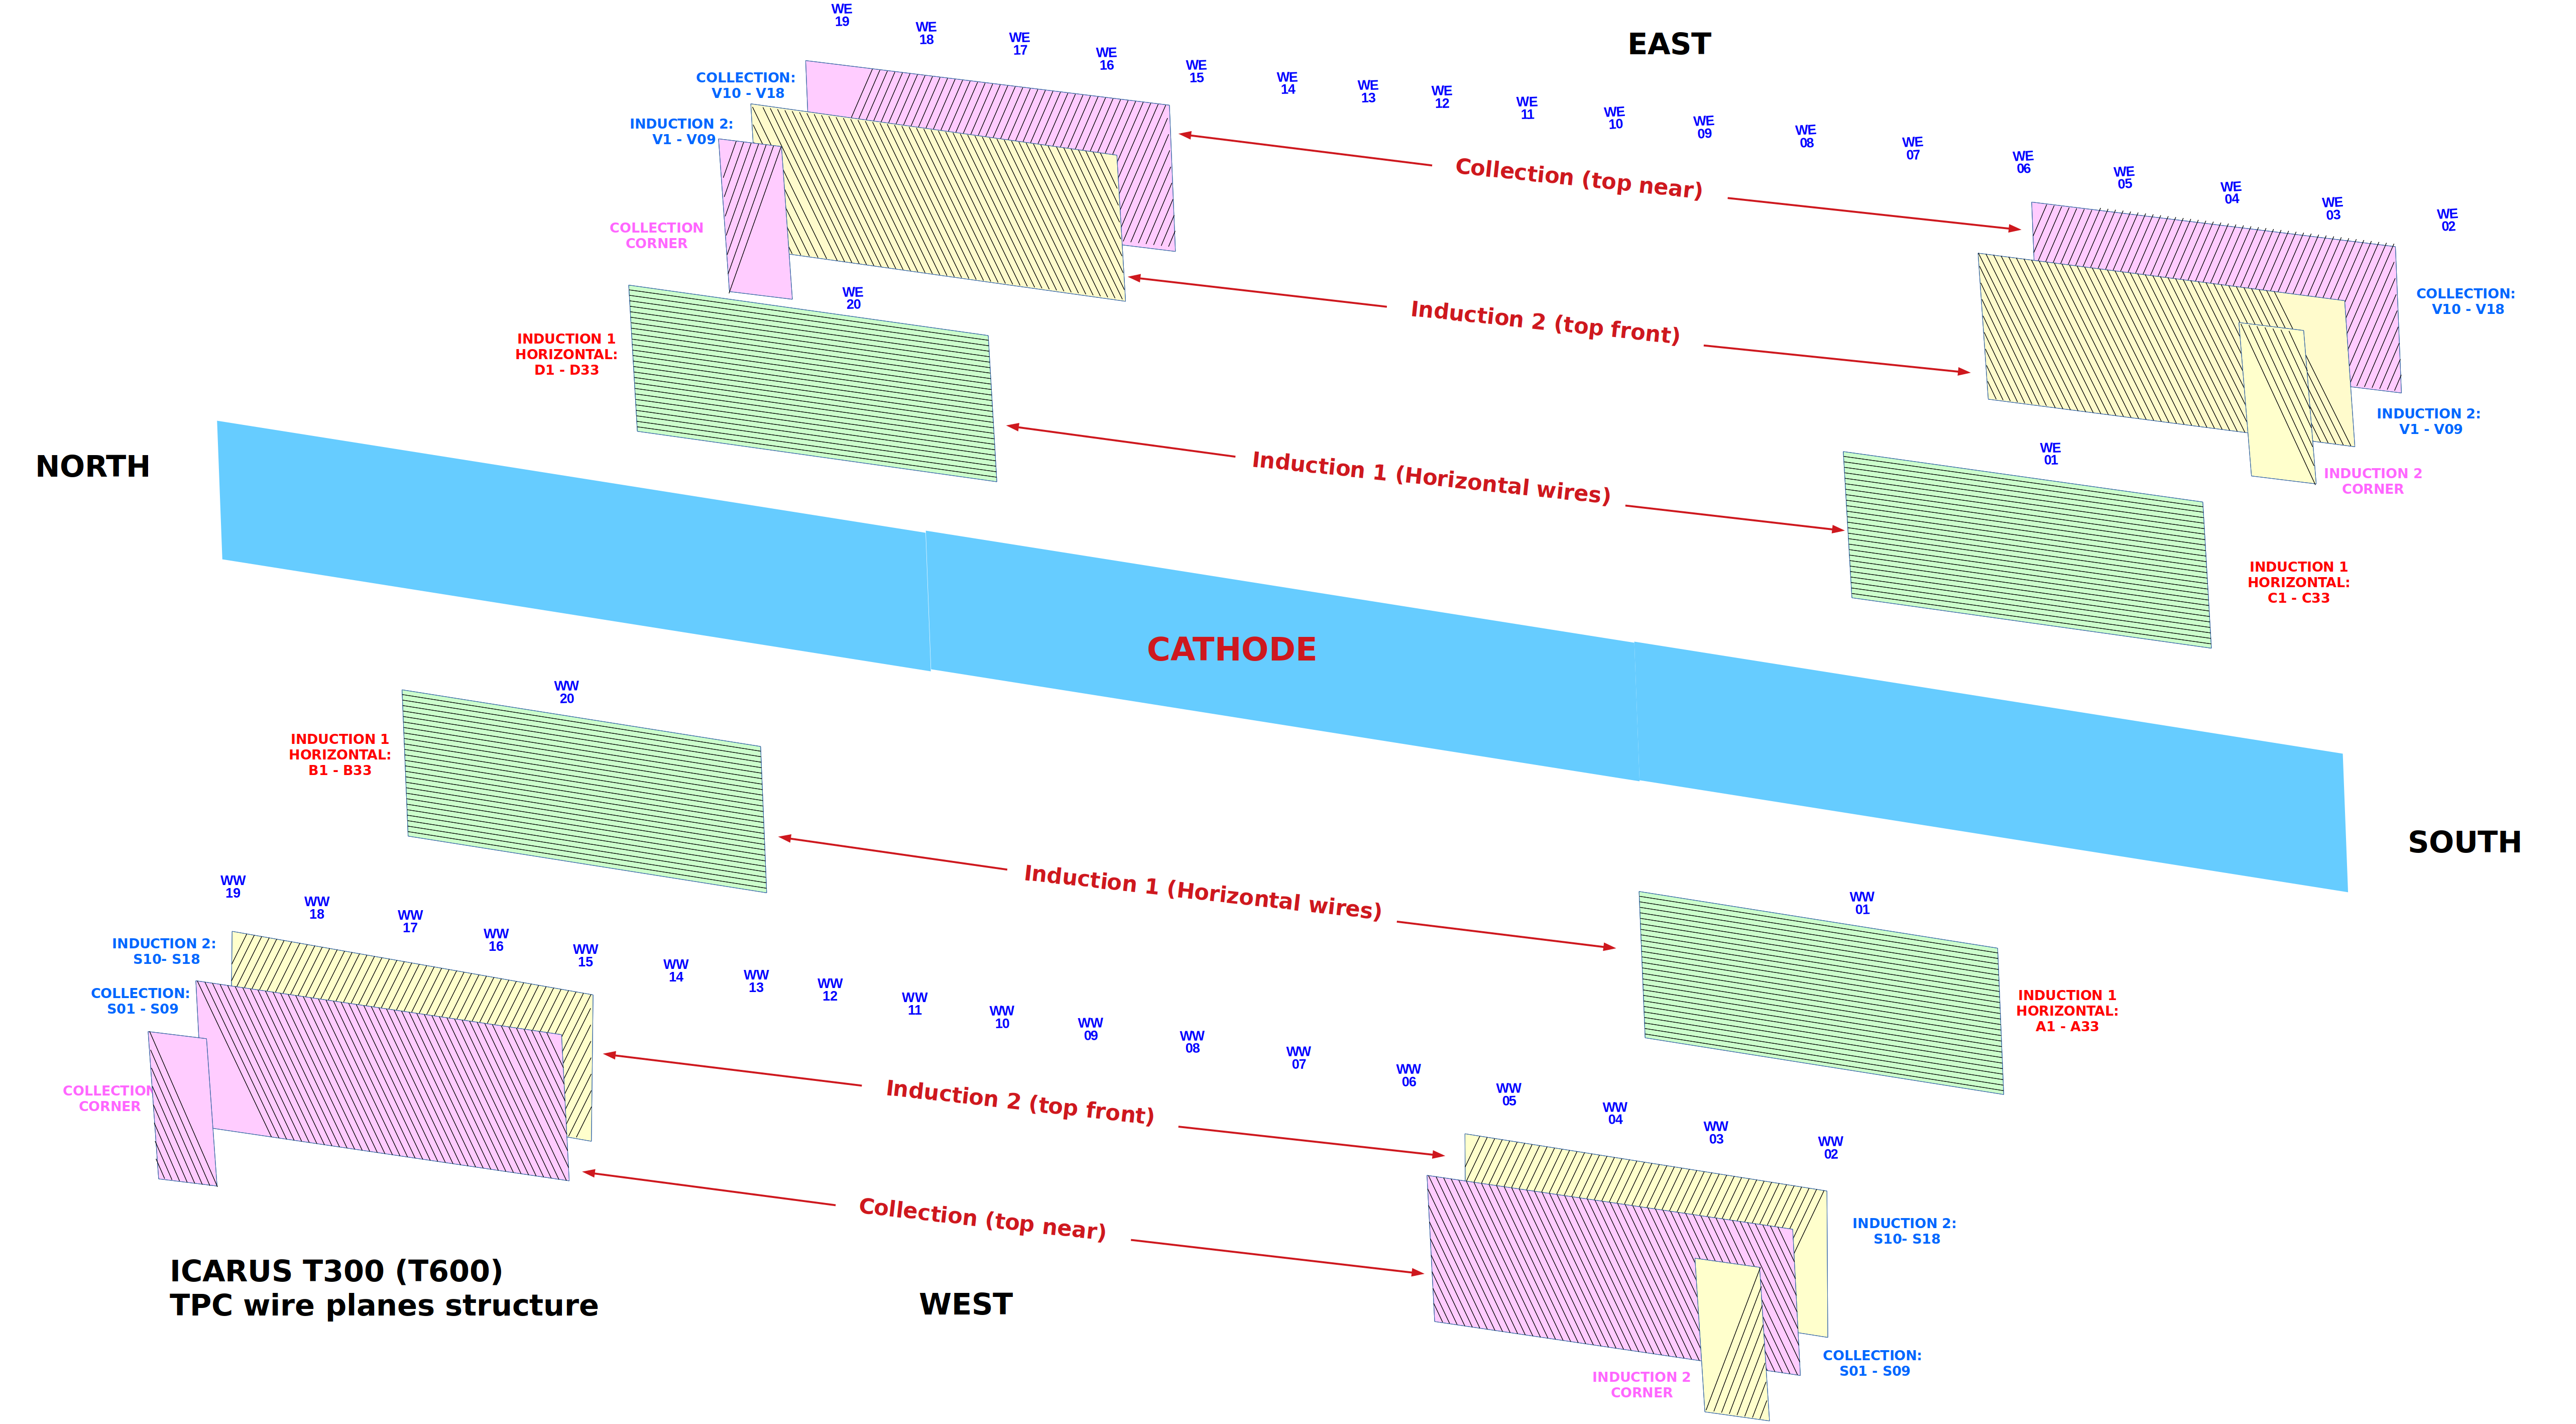
\includegraphics[width=0.90\textheight,angle=90]{figures/Icarus_TPC_wp}}
  \caption{
    Wire planes in a cryostat and their disposition (from~\cite{SBNDocDBxxxx:ConnTest}).
    Note the orientation of the wires, correct and contrasting with the erroneous one in~\cite{SBNDocDB1020}.
    \label{fig:WirePlanesInTPC}
  }
\end{figure}





